% Author of this template: 
%	Felix Schubert
%	schubilab@gmail.com

% Die Quellen werden in zwei verschiedenen .bib-Dateien gespeichert, um so die Internetquellen
% in einem eigenen Verzeichnis führen zu können.

% Die Abkürzungen werden in "latex_einstellungen/akuerzungen/abkuerzungen.tex" geführt.
% Um Veränderungen am Abkürzungsverzeichnis zu übernehmen folgenden Befehl im Terminal ausführen:
% makeindex latex_template.nlo -s nomencl.ist -o latex_template.nls

% Das Deckblatt kann einfach durch das Eigene ersetzt werden. Name muss gleich bleiben!

% Das Template wird laufend verbessert und noch ausführlicher dokumentiert.
% Bei Rückfragen und/ oder Verbesserungsvorschlägen gerne melden.




% Festlegung des Allgemeinen Dokumentenformats
\documentclass[a4paper,12pt,headsepline]{scrartcl}
\usepackage{scrhack}
\usepackage[a4paper, left=4cm, right=2cm, top=4cm, bottom=2cm]{geometry}
\usepackage[scaled=0.90]{helvet}
\usepackage[T1]{fontenc}
\usepackage{courier}
\usepackage[utf8]{inputenc}
\usepackage{graphicx}
\usepackage[ngerman]{babel}
\usepackage[right]{eurosym}
\usepackage{mathptmx}
\usepackage{float}
\usepackage{longtable}
\usepackage{fancybox}
\usepackage{lscape}
\usepackage{pdflscape}
\usepackage[hyphens,obeyspaces,spaces]{url}
\usepackage{color}
\usepackage{amssymb}
\usepackage{fancyhdr} 
\usepackage{array}
\usepackage{multibib}
\usepackage{mathptmx}
\usepackage{multirow}
\usepackage{microtype}
\usepackage{booktabs}
\usepackage[table,xcdraw]{xcolor}
\usepackage{rotating}
\usepackage{caption}
\usepackage{xparse}
\usepackage{lineno}
\usepackage{courier}
\usepackage{paralist}
\usepackage[htt]{hyphenat}
\usepackage{tabularx}
\usepackage{setspace}
\usepackage{capt-of}
\usepackage{makeidx}
\usepackage{pdfpages}
\usepackage{listings}
\lstset{numbers=left, numberstyle=\tiny, numbersep=5pt, keywordstyle=\color{black}\bfseries, stringstyle=\ttfamily,showstringspaces=false,basicstyle=\footnotesize,captionpos=b}
\usepackage{setspace}
\onehalfspacing
\usepackage[german]{nomencl}
\let\abbrev\nomenclature
\usepackage{silence}
\WarningsOff

\newcites{online}{Internetquellen}

\pagestyle{fancy} 
\fancyhf{} 
\fancyhead[L]{\nouppercase{\leftmark}} 
\fancyhead[C]{} 
\fancyhead[R]{\thepage} 
\renewcommand{\headrulewidth}{0.4pt} 

\hbadness=10000
\hfuzz=\maxdimen
\newcount\hbadness
\newdimen\hfuzz
\setlength{\parindent}{0mm}
\setlength{\parskip}{0.8em plus 0.5em minus 0.3em}

\newlength{\transcriptlen}
\NewDocumentCommand {\setspeaker} { mo } {%
	\IfNoValueTF{#2}
	{\expandafter\newcommand\csname#1\endcsname{\item[#1:]}}%
	{\expandafter\newcommand\csname#1\endcsname{\item[#2:]}}%
	\IfNoValueTF{#2}
	{\settowidth{\transcriptlen}{#1}}%
	{\settowidth{\transcriptlen}{#2}}%
}

\makeindex

\renewcommand{\nomname}{Abkürzungsverzeichnis}
\setlength{\nomlabelwidth}{.25\textwidth}
\renewcommand{\nomlabel}[1]{#1 \dotfill}
\setlength{\nomitemsep}{-\parsep}
\makenomenclature

 \widowpenalty = 10000
 \displaywidowpenalty = 1000

\usepackage[pdftex,
bookmarksnumbered,
pdfauthor={Felix Schubert},
pdftitle={Der Bereitstellungsprozess einer digitalen Bauakteneinsicht},
pdfsubject={Bachelor-Thesis},
hyperfootnotes=false]{hyperref}
\hypersetup{colorlinks, citecolor=black, linkcolor= black, urlcolor=black}




\begin{document}

% hier werden die Trennvorschläge inkludiert
%hier müssen alle Wörter rein, welche Latex von sich auch nicht korrekt trennt bzw. bei denen man die genaue Trennung vorgeben möchte
\hyphenation{
Film-pro-du-zen-ten
Lux-em-burg
Soft-ware-bau-steins
zeit-in-ten-siv
Da-ten-schutz-be-auf-trag-ter
Sys-tem-ab-bild
}


\newpage


%FOM_Titelseite
\thispagestyle{empty}

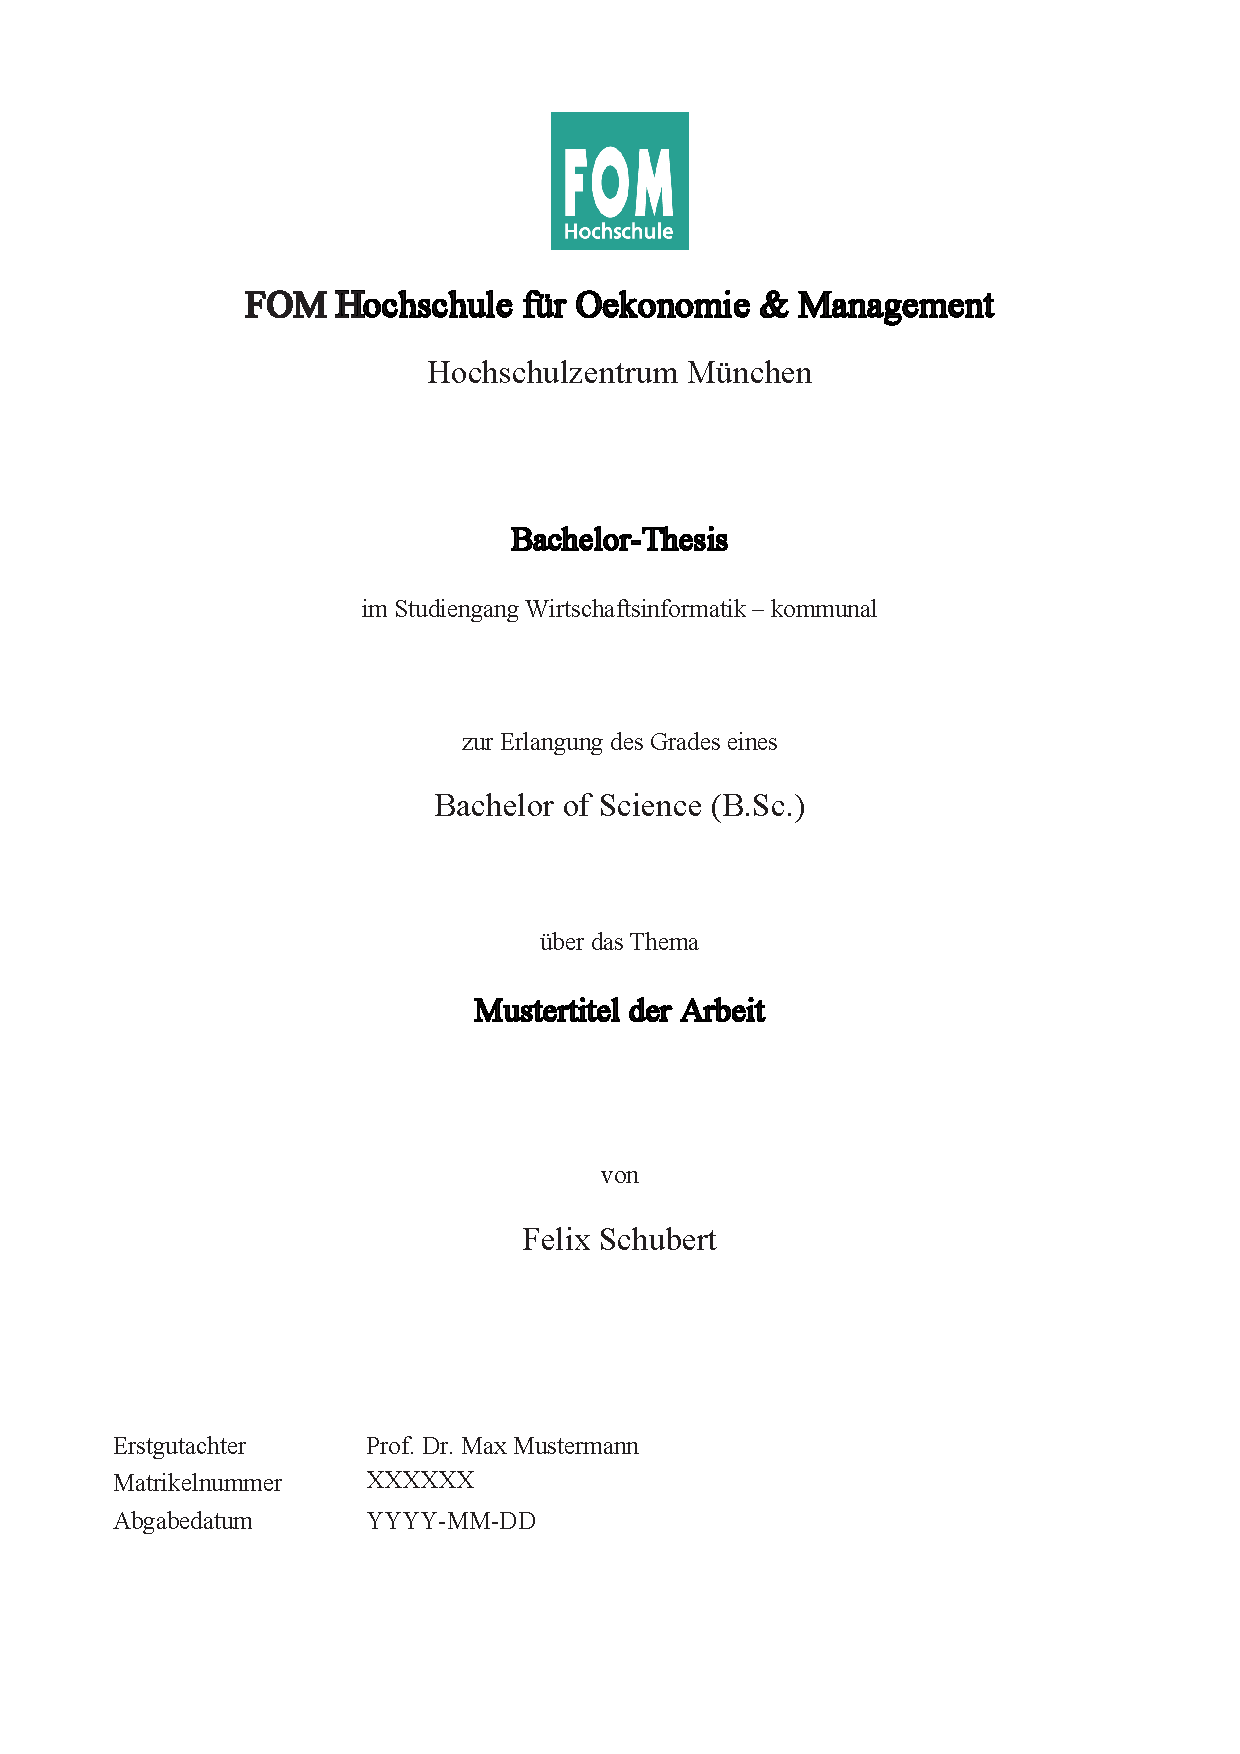
\includepdf{latex_einstellungen/Muster-Deckblatt-Arbeit}

\pagenumbering{Roman}
\setcounter{page}{2}
\onehalfspacing

\thispagestyle{empty}
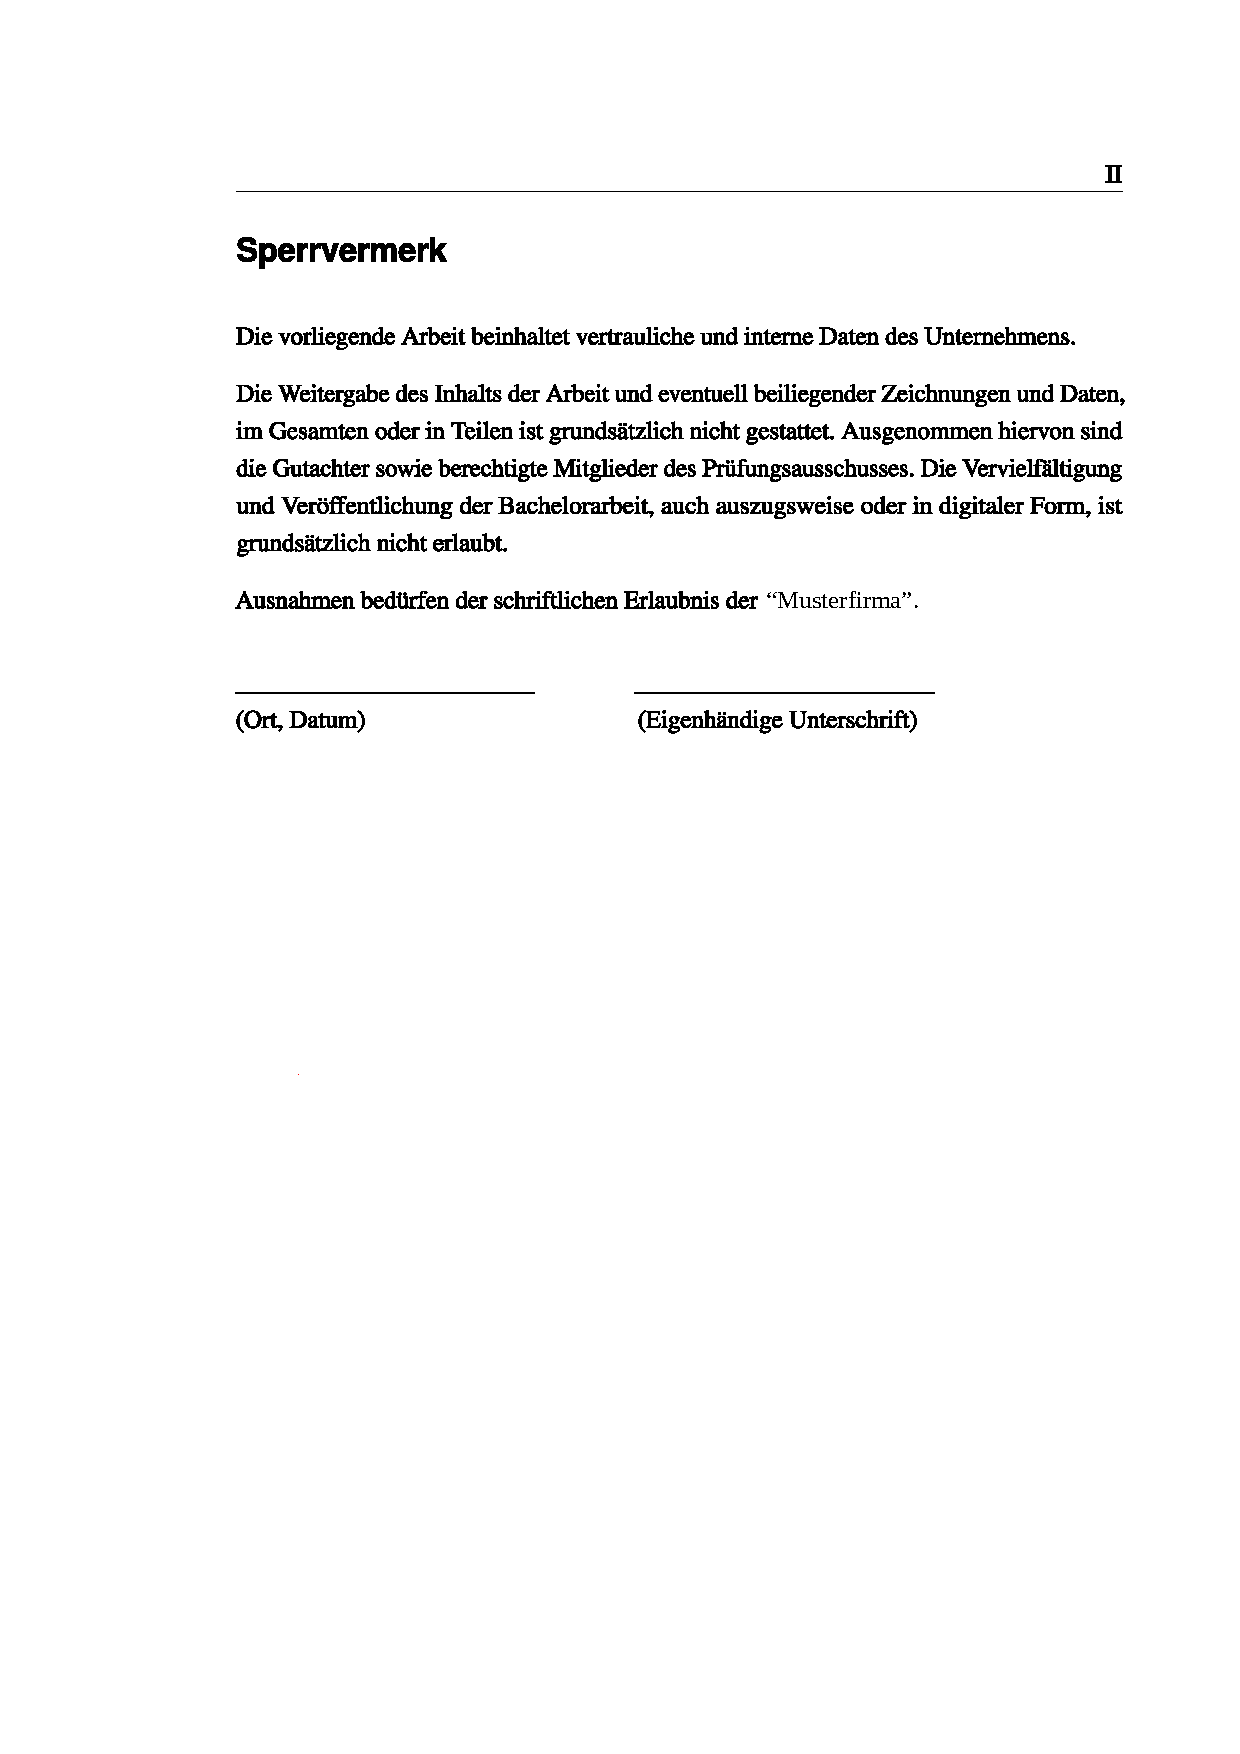
\includepdf{latex_einstellungen/sperrvermerk}
\newpage

% Einleitung / Abstract
\section*{Zusammenfassung}

\textbf{Name des Studierenden}\\
\noindent\hspace*{15mm}%
Felix Schubert
\\
\\
\textbf{Thema der Bachelor-Thesis}\\
\noindent\hspace*{15mm}%
Der Bereitstellungsprozess einer digitalen Bauakteneinsicht
\\
\\
\textbf{Stichworte}\\
\noindent\hspace*{15mm}%
Bauakteneinsicht, Digitalisierung, ProjektPLUS, Systems Engineering
\\
\\
\textbf{Abstract}
\par
\begingroup
\leftskip=15mm % Parameter anpassen
\vspace{-0.33cm}
\noindent %ab hier der Text, der eingerückt werden soll

Lorem ipsum dolor sit amet, consetetur sadipscing elitr, sed diam nonumy eirmod tempor invidunt ut labore et dolore magna aliquyam erat, sed diam voluptua. At vero eos et accusam et justo duo dolores et ea rebum. 

Stet clita kasd gubergren, no sea takimata sanctus est Lorem ipsum dolor sit amet. 

Lorem ipsum dolor sit amet, consetetur sadipscing elitr, sed diam nonumy eirmod tempor invidunt ut labore et dolore magna aliquyam erat, sed diam voluptua. 

At vero eos et accusam et justo duo dolores et ea rebum. Stet clita kasd gubergren, no sea takimata sanctus est Lorem ipsum dolor sit amet.

Lorem ipsum dolor sit amet, consetetur sadipscing elitr, sed diam nonumy eirmod tempor invidunt ut labore et dolore magna aliquyam erat, sed diam voluptua. At vero eos et accusam et justo duo dolores et ea rebum. 

Stet clita kasd gubergren, no sea takimata sanctus est Lorem ipsum dolor sit amet. 

Lorem ipsum dolor sit amet, consetetur sadipscing elitr, sed diam nonumy eirmod tempor invidunt ut labore et dolore magna aliquyam erat, sed diam voluptua. 

At vero eos et accusam et justo duo dolores et ea rebum. Stet clita kasd gubergren, no sea takimata sanctus est Lorem ipsum dolor sit amet.
\par
\endgroup


\singlespacing
\newpage

\tableofcontents
\newpage

\phantomsection
\addcontentsline{toc}{section}{Abbildungsverzeichnis}
\listoffigures
\phantomsection
\addcontentsline{toc}{section}{Tabellenverzeichnis}
\listoftables
\phantomsection
\addcontentsline{toc}{section}{Listingverzeichnis}
\fancyhead[L]{Abbildungs-, Tabellen- und Listingverzeichnis} 
\renewcommand{\lstlistlistingname}{Listingverzeichnis}
\lstlistoflistings
\newpage
\phantomsection
\addcontentsline{toc}{section}{Abkürzungsverzeichnis}
\fancyhead[L]{Abkürzungsverzeichnis} 
\nomenclature{LBK}{Lokalbaukommission}
\nomenclature{LHM}{Landeshauptstadt München}
\nomenclature{IT}{Informationstechnik}
\nomenclature{DAP}{Datenaustauschplattform}
\nomenclature{HTML}{Hypertext Markup Language}
\nomenclature{CSV}{Comma Separated Values}
\nomenclature{PLAN}{Referat für Stadtplanung und Bauordnung}
\nomenclature{ZR}{Zentralregistratur}
\nomenclature{SE}{Systems Engineering}
\nomenclature{Bspw.}{Beispielsweise}
\nomenclature{ODS}{OASIS OpenDocument}
\nomenclature{VBS}{Visual Basic Script}
\nomenclature{GPAM}{Geschäftsprozess- und Anforderungsmanagement}
\nomenclature{PDF}{Portable Document Format}


\printnomenclature[3cm]



%%%%%%% EINLEITUNG %%%%%%%%%%%%

\clearpage
\pagenumbering{arabic}
\newpage
\fancyhead[L]{\nouppercase{\leftmark}} 
\onehalfspacing

% einzelne Abschnitte
\section{Einleitung}

Lorem ipsum dolor sit amet, consetetur sadipscing elitr, sed diam nonumy eirmod tempor invidunt ut labore et dolore magna aliquyam erat, sed diam voluptua. At vero eos et accusam et justo duo dolores et ea rebum. Stet clita kasd gubergren, no sea takimata sanctus est Lorem ipsum dolor sit amet.

% Zweite Gliederungsebende

\subsection{Problemstellung}\label{Problemstellung}

Lorem ipsum dolor sit amet, consetetur sadipscing elitr, sed diam nonumy eirmod tempor invidunt ut labore et dolore magna aliquyam erat, sed diam voluptua.\footnote{Beispiel für eine Fußnote}
 At vero eos et accusam et justo duo dolores et ea rebum.
\subsection{Zielsetzung und Forschungsfrage}\label{Zielsetzung}

Lorem ipsum dolor sit amet, consetetur sadipscing elitr, sed diam nonumy eirmod tempor invidunt ut labore et dolore magna aliquyam erat, sed diam voluptua.

\subsection{Forschungsmethodik}\label{Forschungsmethodik}
Lorem ipsum dolor sit amet, consetetur sadipscing elitr, sed diam nonumy eirmod tempor invidunt ut labore et dolore magna aliquyam erat, sed diam voluptua.
\subsection{Aufbau der Arbeit}

Lorem ipsum dolor sit amet, consetetur sadipscing elitr, sed diam nonumy eirmod tempor invidunt ut labore et dolore magna aliquyam erat, sed diam voluptua. At vero eos et accusam et justo duo dolores et ea rebum. Stet clita kasd gubergren, no sea takimata sanctus est Lorem ipsum dolor sit amet.








\newpage
\section{Die analoge Bauakteneinsicht}\label{Die analoge Bauakteneinsicht}

Lorem ipsum dolor sit amet, consetetur sadipscing elitr, sed diam nonumy eirmod tempor invidunt ut labore et dolore magna aliquyam erat, sed diam voluptua. At vero eos et accusam et justo duo dolores et ea rebum. Stet clita kasd gubergren, no sea takimata sanctus est Lorem ipsum dolor sit amet.

\subsection{Stärken, Schwächen, Chancen und Risiken}\label{SWOT-Analyse}

Lorem ipsum dolor sit amet, consetetur sadipscing elitr, sed diam nonumy eirmod tempor invidunt ut labore et dolore magna aliquyam erat, sed diam voluptua. At vero eos et accusam et justo duo dolores et ea rebum. Stet clita kasd gubergren, no sea takimata sanctus est Lorem ipsum dolor sit amet.
\subsection{Die gesetzlichen Herausforderungen}\label{Gesetzliche_Herausforderungen}

Lorem ipsum dolor sit amet, consetetur sadipscing elitr, sed diam nonumy eirmod tempor invidunt ut labore et dolore magna aliquyam erat, sed diam voluptua. At vero eos et accusam et justo duo dolores et ea rebum. Stet clita kasd gubergren, no sea takimata sanctus est Lorem ipsum dolor sit amet.





\newpage
\section{Rahmenbedingungen}\label{Rahmenbedingungen}

Lorem ipsum dolor sit amet, consetetur sadipscing elitr, sed diam nonumy eirmod tempor invidunt ut labore et dolore magna aliquyam erat, sed diam voluptua. At vero eos et accusam et justo duo dolores et ea rebum. Stet clita kasd gubergren, no sea takimata sanctus est Lorem ipsum dolor sit amet. Stet clita kasd gubergren, no sea takimata sanctus est Lorem ipsum dolor sit amet.

\subsection{Hier werden die Quellen angezeigt}

Onlinequelle: \citeonline{Panitz2017}

E-Mail: \citeonline{Schubert2019}

Quelle mit Seitenzahl: \cite[S. 2 f.]{Vaughan2016}


\subsection{Abbildungen}

\begin{figure}[H]
	\centering
	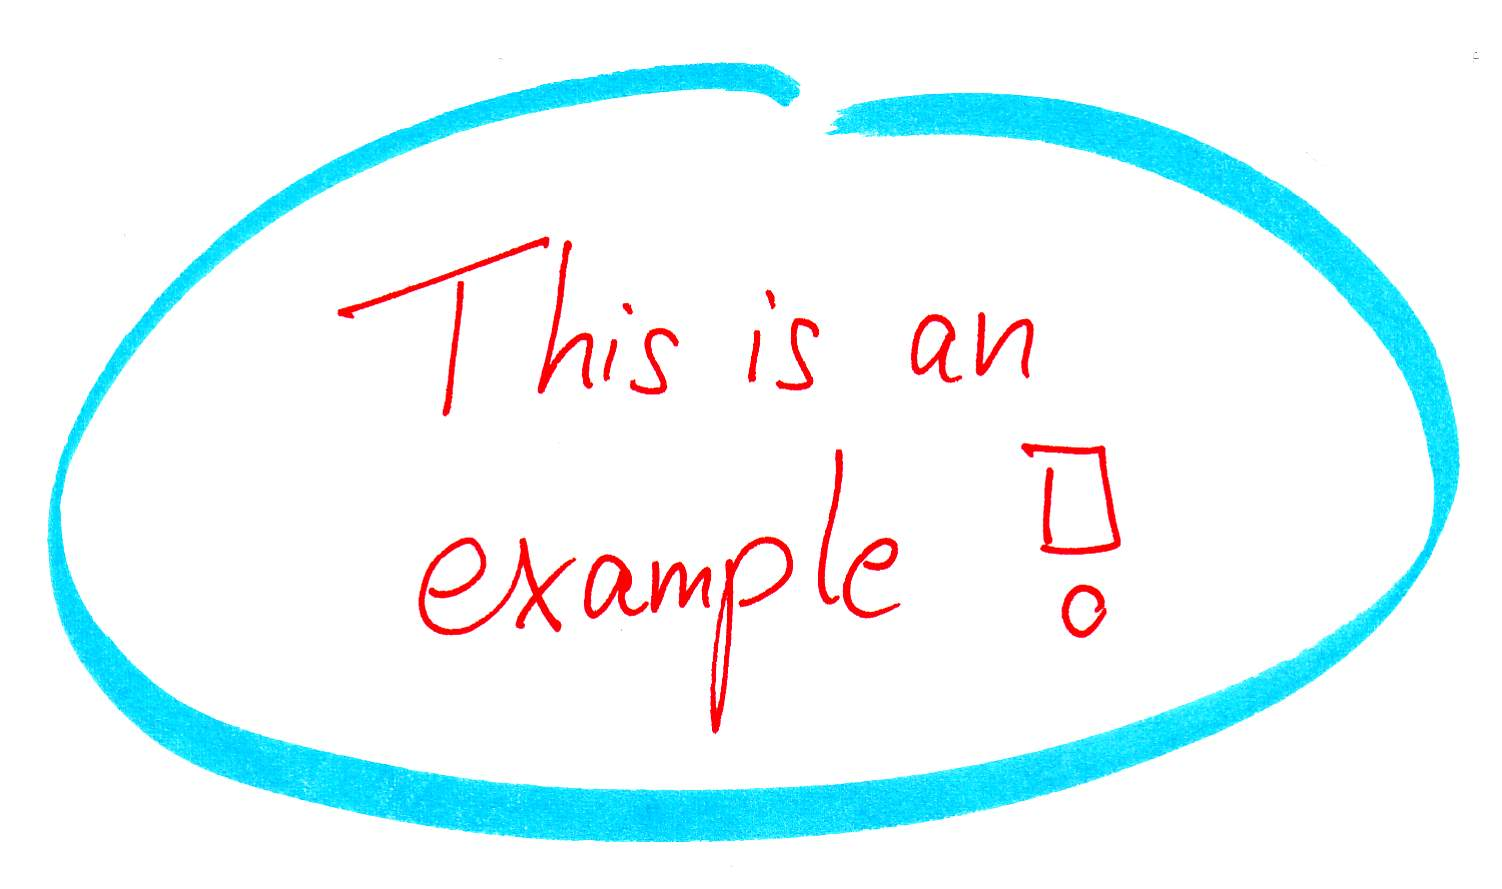
\includegraphics[width=15cm]{bilder/example.jpg}
	\caption{Example}
	\label{abb:example}
	Quelle: \url{https://ftp.fau.de/ctan/macros/latex/contrib/incgraph/example.jpg}
\end{figure}


\subsection{Tabellen}

Nachfolgend ein Beispiel einer Tabelle.
\begin{center}
		\begin{tabular}{l|ll}
		SWOT  & positiv & negativ   \\ \hline
		innen & Stärken & Schwächen \\
		außen & Chancen & Risiken  
		\end{tabular}
		\captionof{table}{Die SWOT-Analyse}
		Quelle: Eigenentwicklung
		\label{tab:swot-analyse}  
\end{center}
	






\subsection{Listings}

Nachfolgend ein Code-Beispiel.

\begin{lstlisting}[caption={Hello World in C}]
	#include<stdio.h>

	int main() {
		printf("Hello World\n");
		return 0;
	}
\end{lstlisting}
	









\newpage
% \input{Kapitel/04_Kapitel_4/04_main}
% \newpage
% \input{Kapitel/05_Kapitel_5/05_main}
% \newpage
%\input{07_fazit_und_ausblick/7_0}
%..

\singlespacing
\newpage
\phantomsection
\addcontentsline{toc}{section}{Literaturverzeichnis}
\renewcommand\refname{Literaturverzeichnis}
\bibliographystyle{alphadin_edit_fs}
\bibliography{sources}
\newpage

\phantomsection
\addcontentsline{toc}{section}{Internetquellen}
\renewcommand\refname{Internetquellen}
\bibliographystyleonline{alphadin_edit_fs}
\bibliographyonline{online_sources}
\onehalfspacing
\newpage

\phantomsection
\addcontentsline{toc}{section}{Anhang}
\renewcommand\refname{Anhang}
\fancyhead[L]{Anhang} 
%\subsection*{Anhang}\label{anhang}

%Um im Inhaltsverzeichnis einen Eintrag zu erzeugen
%\section*{Anhangsverzeichnis}

\appendix
\renewcommand*{\thesection}{A\arabic{section}}
% Set the name for the list of appenices
\newcommand\listoftoaname{Anhang}

% force table of contents to load the list of appendices
\let\oldlistoftoc\listoftoc
\renewcommand\listoftoc[1]{\oldlistoftoc{toa}}
\tableofcontents
\let\listoftoc\oldlistoftoc  
% we will now redefine the sectioning commands so that that put entries
% into the list of appendices. The redefinitions are rather simplistic
% and break the starred versions and the optional argument.
% Thus the redefinitions have to be added after the \tableofcontents call.

\let\oldaddcontentsline\addcontentsline
\newcommand\hackedaddcontentsline[3]{\oldaddcontentsline{toa}{#2}{#3}}

\let\oldsection\section
\renewcommand*\section[1]{%
	\let\addcontentsline\hackedaddcontentsline%
	\oldsection{#1}%
	\let\addcontentsline\oldaddcontentsline%
}

\let\oldsubsection\subsection
\renewcommand*\subsection[1]{%
	\let\addcontentsline\hackedaddcontentsline%
	\oldsubsection{#1}%
	\let\addcontentsline\oldaddcontentsline%
}

\let\oldsubsubsection\subsubsection
\renewcommand*\subsubsection[1]{%
	\let\addcontentsline\hackedaddcontentsline%
	\oldsubsubsection{#1}%
	\let\addcontentsline\oldaddcontentsline%
}

\newpage

%REFERENZEN kontrollieren
\begin{appendix}

	\section{Interviews}\label{Interviews_Anhang}
	\addcontentsline{toc}{section}{A. Interviews}
	\subsection{Die datenschutzrechtlichen Aspekte einer digitalen Bauakteneinsicht}
\addcontentsline{toc}{subsection}{A.2. Die datenschutzrechtlichen Aspekte einer digitalen Bauakteneinsicht}
% Easiest to put the longest name last...

Interviewer: Felix Schubert\\
Befragter: Max Mustermann

Datum: 16.04.2020
\label{interview_data}
	
\newcolumntype{R}[1]{>{\raggedleft\arraybackslash}p{#1}}
\newcolumntype{C}[1]{>{\centering\arraybackslash}p{#1}}
\setspeaker{B}
\setspeaker{I}
 
% How much of a gap between speakers and text?
\addtolength{\transcriptlen}{1em}%

\linenumbers[1]


	\begin{description}
		
	\I Lorem ipsum dolor sit amet, consetetur sadipscing elitr, sed diam nonumy eirmod tempor invidunt ut labore et dolore magna aliquyam erat, sed diam voluptua. 00:00:23-1
	\B Lorem ipsum dolor sit amet, consetetur sadipscing elitr, sed diam nonumy eirmod tempor invidunt ut labore et dolore magna aliquyam erat, sed diam voluptua. 00:00:55-2
	\item Kurze Unterbrechung 
	\I Lorem ipsum dolor sit amet, consetetur sadipscing elitr, sed diam nonumy eirmod tempor invidunt ut labore et dolore magna aliquyam erat, sed diam voluptua. 00:01:35-3
	\B Ende des Interviews. 00:01:55-4

		
	\end{description}
\nolinenumbers
	\newpage
	\subsection{Die rechtlichen Aspekte einer digitalen Bauakteneinsicht}
\addcontentsline{toc}{subsection}{A.2. Die rechtlichen Aspekte einer digitalen Bauakteneinsicht}
% Easiest to put the longest name last...

Interviewer: Felix Schubert\\
Befragter: Martine Mustermann

Datum: 22.04.2020
\label{interview_data}
	
\newcolumntype{R}[1]{>{\raggedleft\arraybackslash}p{#1}}
\newcolumntype{C}[1]{>{\centering\arraybackslash}p{#1}}
\setspeaker{B2}
\setspeaker{I2}
 
% How much of a gap between speakers and text?
\addtolength{\transcriptlen}{1em}%

\linenumbers[1]


	\begin{description}
		
	\I2 Lorem ipsum dolor sit amet, consetetur sadipscing elitr, sed diam nonumy eirmod tempor invidunt ut labore et dolore magna aliquyam erat, sed diam voluptua. 00:00:23-1
	\B2 Lorem ipsum dolor sit amet, consetetur sadipscing elitr, sed diam nonumy eirmod tempor invidunt ut labore et dolore magna aliquyam erat, sed diam voluptua. 00:00:55-2
	\item Kurze Unterbrechung 
	\I2 Lorem ipsum dolor sit amet, consetetur sadipscing elitr, sed diam nonumy eirmod tempor invidunt ut labore et dolore magna aliquyam erat, sed diam voluptua. 00:01:35-3
	\B2 Ende des Interviews. 00:01:55-4

		
	\end{description}
\nolinenumbers
	\newpage	

	\section{Abbildungen}
	\addcontentsline{toc}{section}{B. Abbildungen}
	

In diesem Abschnitt des Anhangs werden die Abbildungen dargestellt, welche im Text referenziert wurden.







%\newpage
%
%\subsection{Terminal Standort, Entscheidungsmatrix}



\begin{figure}[H]
	\centering
	
\includegraphics[width=15cm]{anhaenge/abbildungen/the_latex_project.png}
	\caption[]{Quick Wins}
	\label{abb:quick_win}
	Quelle: \url{https://en.wikipedia.org/wiki/LaTeX#/media/File:LaTeX_project_logo_bird.svg}
\end{figure}



	\newpage	
	\section{Tabellen}
	\addcontentsline{toc}{section}{C. Tabellen}
	Lorem ipsum dolor sit amet, consetetur sadipscing elitr, sed diam nonumy eirmod tempor invidunt ut labore et dolore magna aliquyam erat, sed diam voluptua. At vero eos et accusam et justo duo dolores et ea rebum. \\
Anbei ein Beispiel einer Tabelle:


\begin{small}
	\begin{longtable}{|p{6.5cm}|p{1.5cm}|p{2.5cm}|p{2.5cm}|}

	\hline
	\rowcolor[gray]{.8} Vorgangsname & Dauer & Anfang & Ende \\
		\hline
		\endfirsthead
		\multicolumn{3}{c}%	
		{{\bfseries Fortsetzung des Projektablaufplans.}} \\
		\hline
		\rowcolor[gray]{.8} Vorgangsname & Dauer & Anfang & Ende \\ 
		\hline
		\endhead
		
		
		\textbf{Lorem ipsum dolor} & \textbf{281 Tage} & \textbf{Don 28.02.19} & \textbf{Don 30.04.20} \\
		 \hline
		\textbf{   Projektvorbereitung} & \textbf{29 Tage} & \textbf{Don 28.02.19} & \textbf{Die 09.04.19} \\
		 \hline
		\textbf{      I. Meilenstein: Lorem ipsum dolor sit amet} & 0 Tage & Don 28.02.19 & Don 28.02.19 \\
		 \hline
		 Lorem ipsum dolor sit amet & 3 Tage & Mon 11.03.19 & Mit 13.03.19 \\
		 \hline
		 Lorem ipsum dolor sit amet & 1 Tag & Mit 13.03.19 & Mit 13.03.19 \\
		 \hline
		 Lorem ipsum dolor sit amet & 1 Tag & Mon 18.03.19 & Mon 18.03.19 \\
		 \hline
		 Lorem ipsum dolor sit amet & 1 Tag & Mon 25.03.19 & Mon 25.03.19 \\
		 \hline
		 Lorem ipsum dolor sit amet & 1 Tag & Mon 25.03.19 & Mon 25.03.19 \\
		 \hline
		\textbf{      II. Meilenstein: Lorem ipsum dolor sit amet,} & 0 Tage & Mon 25.03.19 & Mon 25.03.19 \\
		 \hline
		 Lorem ipsum dolor sit amet & 1 Tag & Mon 25.03.19 & Mon 25.03.19 \\
		 \hline
		 Lorem ipsum dolor sit amet & 1 Tag & Die 26.03.19 & Die 26.03.19 \\
		 \hline
		 Lorem ipsum dolor sit amet & 1 Tag & Die 26.03.19 & Die 26.03.19 \\
		 \hline
		 Lorem ipsum dolor sit amet & 1 Tag & Don 28.03.19 & Don 28.03.19 \\
		 \hline
		 Lorem ipsum dolor sit amet & 1 Tag & Die 02.04.19 & Die 02.04.19 \\
		\hline	
		\caption*{Tabelle: Projektablaufplan}
		\label{tab:Projektablaufplan}  \\
	\end{longtable}%
\vspace{-1.5cm}
\begin{center}
{\normalsize 	Quelle: Eigenentwicklung}
\end{center}
	
\end{small}



\begin{landscape}
	
Das ist ein Beispiel einer waagerechten Seite.
	
\end{landscape}







	\newpage
	
\end{appendix}



\begin{figure}[H]
\centering
	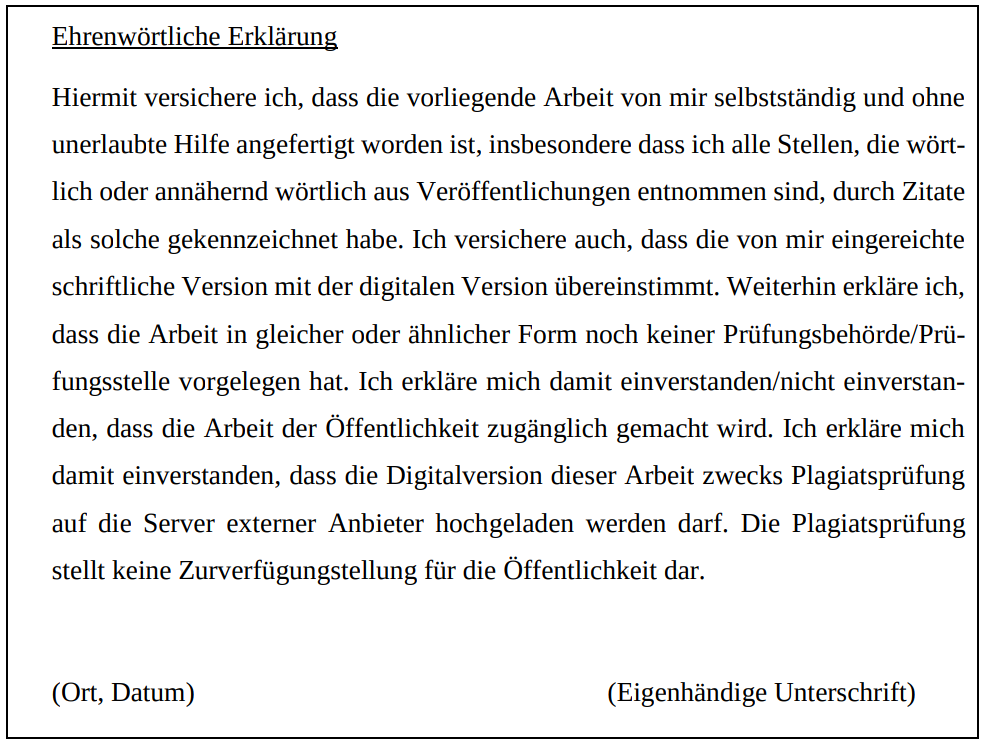
\includegraphics[width=\textwidth]{latex_einstellungen/ehrenwoertliche_erklaerung/ehren_erklaerung.png}
\end{figure}


\mbox{}
\end{document}